\documentclass[
11pt,						% Schriftgröße
DIV10,
german,						% für Umlaute, Silbentrennung etc.
paper=a4,					% Papierformat
oneside,
titlepage,					% es wird eine Titelseite verwendet
parskip=half,				% Abstand zwischen Absätzen (halbe Zeile)
headings=normal,			% Größe der Überschriften verkleinern
listof=totoc,				% Verzeichnisse im Inhaltsverzeichnis aufführen
bibliography=totoc,			% Literaturverzeichnis im Inhaltsverzeichnis aufführen
numbers=noenddot,			% Kapitelnummern ohne Punkt		
]{scrreprt}

\usepackage[utf8]{inputenc}
% Informationen ------------------------------------------------------------
% 	Definition von globalen Parametern, die im gesamten Dokument verwendet
% 	werden können (z.B auf dem Deckblatt etc.).
% --------------------------------------------------------------------------
\newcommand{\titel}{Kartenspiel Uno}
\newcommand{\untertitel}{Softwareengineering Projekt}
\newcommand{\semester}{-}
\newcommand{\art}{Vorlage}
\newcommand{\autor}{Felix Bauer}
\newcommand{\matrikel}{695033}
\newcommand{\studienbereich}{Elektrotechnik}
\newcommand{\erstgutachter}{Ludger Winkels}
%\newcommand{\zweitgutachter}{}
\newcommand{\jahr}{2022}

% Eigene Befehle
%\newcommand{\todo}[1]{\textbf{\textsc{\textcolor{red}{(TODO: #1)}}}}
\newcommand{\todo}[1]{\textcolor{red}{(TODO:#1)}}
% Autorennamen in small caps
\newcommand{\AutorZ}[1]{\textsc{#1}}
\newcommand{\Autor}[1]{\AutorZ{\citeauthor{#1}}}

% Befehle zur semantischen Auszeichnung von Text
\newcommand{\NeuerBegriff}[1]{\textbf{#1}}
\newcommand{\Fachbegriff}[1]{\textit{#1}}
\newcommand{\Prozess}[1]{\textit{#1}}
\newcommand{\Webservice}[1]{\textit{#1}}
\newcommand{\Eingabe}[1]{\texttt{#1}}
\newcommand{\Code}[1]{\texttt{#1}}
\newcommand{\Datei}[1]{\texttt{#1}}
\newcommand{\Datentyp}[1]{\textsf{#1}}
\newcommand{\XMLElement}[1]{\textsf{#1}}

% Abkürzungen
\newcommand{\vgl}[1]{\mbox{vgl.~#1}}
\newcommand{\ua}{\mbox{u.\,a.\ }}
\newcommand{\zB}{\mbox{z.\,B.\ }}
\newcommand{\siehe}[1]{\mbox{s.~#1}}
\newcommand{\nach}[1]{\mbox{nach~#1}}
\newcommand{\mathe}[1][black]{$\mathrm{#1}$}
\newcommand{\hervorheben}{\rowcolor[gray]{0.95}}

\newcommand{\afz}[1]{,,#1''}
% Anpassung des Seitenlayouts ----------------------------------------------
% 	siehe Seitenstil.tex
% --------------------------------------------------------------------------
\usepackage[headsepline,automark]{scrlayer-scrpage}

\usepackage[table]{xcolor} 
\definecolor{colBackground}{rgb}{0.95, 0.95, 0.95}
\definecolor{colKeyword}{rgb}{0, 0, 0.9}
\definecolor{colComment}{rgb}{0, 0.6, 0}
\definecolor{colString}{rgb}{0.8, 0, 0}

\usepackage{listingsutf8}
\lstset{language=C++,
	basicstyle =\footnotesize\selectfont\ttfamily,
	backgroundcolor=\color{colBackground},
	keywordstyle=\color{colKeyword},
	stringstyle=\color{colString},
	showstringspaces=false,
	commentstyle=\color{colComment},
	breaklines=true,
	numbers=left,
	stepnumber=1,
	numbersep=10pt,
	tabsize=2,
	captionpos=b,
	extendedchars=true,
	frame=single,
	captionpos=t
}

\renewcommand{\lstlistingname}{Codeausschnitt} % Damit Codebeispiele mit Code betitelt werden.



% Anpassung an Landessprache -----------------------------------------------
% 	Verwendet globale Option german siehe \documentclass
% --------------------------------------------------------------------------
\usepackage[ngerman]{babel}
\usepackage{pifont}

\usepackage[utf8]{inputenc}
\usepackage{amsmath,amssymb,units}
\usepackage{esvect}
\usepackage{wrapfig,caption, placeins}
\captionsetup{
	format = plain,
	justification = centering,
	labelsep = newline,
	singlelinecheck = false,
	labelfont = bf,
	font = small
}
\usepackage{mathptmx,charter,helvet,courier}
\usepackage[printonlyused]{acronym}
\usepackage{wrapfig}

% Umlaute ------------------------------------------------------------------
% 		Umlaute/Sonderzeichen wie äöüß direkt im Quelltext verwenden (CodePage).
%		Erlaubt automatische Trennung von Worten mit Umlauten.
% --------------------------------------------------------------------------
\usepackage[utf8]{inputenc}
\usepackage[T1]{fontenc}
\usepackage{ae}			 	% "schöneres" ä
\usepackage{textcomp} 		% Euro-Zeichen etc.
\usepackage[german=quotes]{csquotes}



% Verwendung von Blindtext zur Layout gestaltung -----------------------------------------------------
\usepackage{blindtext}

% Grafiken -----------------------------------------------------------------
% 		Einbinden von Grafiken [draft oder final]
% 		Option [draft] bindet Bilder nicht ein - auch globale Option
% --------------------------------------------------------------------------
\usepackage{graphicx}
\graphicspath{{Bilder/}} 	% Dort liegen die Bilder des Dokuments
\usepackage{subcaption}

% Befehle aus AMSTeX für mathematische Symbole z.B. \boldsymbol \mathbb ----
\usepackage{amsmath,amsfonts}

% Für Index-Ausgabe; \printindex -------------------------------------------
\usepackage{makeidx}

% Einfache Definition der Zeilenabstände und Seitenränder etc. -------------
\usepackage{setspace}
\usepackage{geometry}


%% Zum Umfließen von Bildern -------------------------------------------------
\usepackage{floatflt}


% Lange URLs umbrechen etc. -------------------------------------------------
\usepackage{url}

% f�r lange Tabellen
\usepackage{longtable}
\usepackage{array}
\usepackage{ragged2e}
\usepackage{lscape}
\usepackage{colortbl} %farbige hinterlegung


% Spaltendefinition rechtsbündig mit definierter Breite ---------------------
\newcolumntype{w}[1]{>{\raggedleft\hspace{0pt}}p{#1}}

% Formatierung von Listen ändern
\usepackage{paralist}
% Standardeinstellungen:
\setdefaultleftmargin{2.5em}{2.2em}{1.87em}{1.7em}{1em}{1em}

%Zur Verwendung von BibLaTex
%\usepackage[style=numeric]{biblatex}
%\addbibresource{literatur}

% Zur Richtigen Verwendung von Einheiten
\usepackage[locale=DE]{siunitx}

\sisetup{
	mode = text,
	detect-family,
	detect-weight,  
	exponent-product = \cdot,
	number-unit-separator=\text{\,},
	output-decimal-marker={\text{,}},
	%math-rm=\mathsf,
	%text-rm=\sffamily,
	range-phrase = { - }	
}
\DeclareSIUnit{\var}{var}

\usepackage{xcolor}
\usepackage{caption}
\usepackage{float}
%\usepackage{subfig}


% pdf-Optionen  --------------------------------------------------------------
\usepackage[
bookmarks,
bookmarksopen=true,
pdftitle={\titel},
pdfauthor={\autor},
pdfcreator={\autor},
pdfsubject={\titel},
pdfkeywords={\titel},
colorlinks=true,
%linkcolor=red, % einfache interne Verknüpfungen
%anchorcolor=black,% Ankertext
%citecolor=blue, % Verweise auf Literaturverzeichniseinträge im Text
%filecolor=magenta, % Verkn�pfungen, die lokale Dateien �ffnen
%menucolor=red, % Acrobat-Men�punkte
%urlcolor=cyan, 
% f�r die Druckversion k�nnen die Farben ausgeschaltet werden:
linkcolor=black, % einfache interne Verkn�pfungen
anchorcolor=black,% Ankertext
citecolor=black, % Verweise auf Literaturverzeichniseintr�ge im Text
filecolor=black, % Verkn�pfungen, die lokale Dateien �ffnen
menucolor=black, % Acrobat-Men�punkte
urlcolor=black, 
%backref,
%pagebackref,
plainpages=false,% zur korrekten Erstellung der Bookmarks
pdfpagelabels,% zur korrekten Erstellung der Bookmarks
hypertexnames=false,% zur korrekten Erstellung der Bookmarks
linktoc=all%Sowohl Seitenzahl als auch Text als Link
]{hyperref}

\addto\extrasngerman{\def
\subsectionautorefname{Kapitel}
} %Definition "Kapitel" bei autoref von subsection
% Zeilenabstand 1,5 --------------------------------------------------------
\onehalfspacing


% Seitenränder -------------------------------------------------------------
\geometry{paper=a4paper,left=25mm,right=25mm,top=30mm,bottom=40mm}

% Chapter weiter oben beginnen lassen
\renewcommand*\chapterheadstartvskip{\vspace*{0cm}}

% Kopf- und Fußzeilen ------------------------------------------------------
\pagestyle{scrheadings}

% Kopf- und Fußzeile auch auf Kapitelanfangsseiten -------------------------
\renewcommand*{\chapterpagestyle}{scrheadings}

% Schriftform der Kopfzeile ------------------------------------------------
\renewcommand{\headfont}{\normalfont}

% Kopfzeile ----------------------------------------------------------------
\ihead{
	%\parbox{10.0cm}{\normalsize{\titel}}\\
	%\small{\untertitel}\\[2ex]
	\textit{ \headmark}
}
\chead{
		%\includegraphics[height=1.4cm]{Grafiken/firma}
}
\ohead{	
	%\includegraphics[height=1.4cm]{Grafiken/ZF_Logo}
	%\includegraphics[height=1.4cm]{Grafiken/Logo_PHWT.png}	
}
\setlength{\headheight}{21mm} % Höhe der Kopfzeile


% Fußzeile -----------------------------------------------------------------
\ifoot{
	%\includegraphics[height=1.5cm]{Grafiken/Logo_PHWT.png}
}
\cfoot{}
\ofoot{\pagemark}
\setlength{\footheight}{15mm}


% erzeugt ein wenig mehr Platz hinter einem Punkt --------------------------
%\frenchspacing 

% Schusterjungen und Hurenkinder vermeiden
\clubpenalty = 10000
\widowpenalty = 10000 
\displaywidowpenalty = 10000


%% Fußnoten fortlaufend durchnummerieren ------------------------------------
%\counterwithout{footnote}{chapter}
\setkomafont{section}{\large} 




\begin{document}
	
\setcounter{tocdepth}{2} % Tiefe des Inhaltsverzeichnisses definiert

\thispagestyle{plain}
\begin{titlepage}
	
	\begin{center}
		
		\begin{minipage}{0.5\textwidth}
			\centering
			%\includegraphics[height=5cm]{Grafiken/ZF_Logo}
		\end{minipage}%
		\hfill%
		\begin{minipage}{0.5\textwidth}
			\centering
			%\includegraphics[width=7cm]{Grafiken/Logo_PHWT}
		\end{minipage}\\[6ex]
		
		\huge{\textsc{\textbf{\untertitel}}}\\[1.5ex]
		\LARGE{,,\titel''}\\[4ex]		
%		\hbox{
%		\vfill

		\normalsize
		Hochschule für angewandte Wissenschaft und Kunst Göttingen
			
%			}
%	\LARGE{\textbf{\art}}		
	
	\vfill
		\normalsize
		\begin{tabular}{w{5.4cm}p{10cm}}
			vorgelegt von:  & \quad Felix Bauer  \\
			Matrikelnummer:	 & \quad \matrikel	\\	 
			%Studienbereich:  & \quad \studienbereich \\
			Studiengang:     & \quad Elektrotechnik \\   
			Prüfer:      & \quad \erstgutachter \\
			%                 & \quad PHWT \\
			%Zweitprüfer:     & \quad \zweitgutachter \\
			 %                & \quad ZF Friedrichshafen AG \\
			%Bearbeitungszeitraum: & \quad 19.11.2021 - 04.02.2022 \\
		\end{tabular}
		\vfill
		%\copyright\ \jahr\\[1.5ex]
		
	\end{center}
	
\end{titlepage}

\clearpage
\pagenumbering{Roman}
\tableofcontents
\listoffigures
%\listoftables
%\input{Abkuerzungen.tex}

\newpage
\pagenumbering{arabic}


% Einbinden der content Datein
%\input{Kapitel/.tex}
%!TEX root = Uno-Dokumentation.tex
\chapter{Einleitung}
Software wird durch die stetig wachsenden Möglichkeiten immer wichtiger und komplexer. Automatisierungen und Virtualisierungen werden immer mehr eingesetzt und bieten durch ihre hohe Komplexität eine echte Alternative zur Arbeit von Menschenhand. Auch die Videospielindustrie wächst immer weiter und erfreut sich immer mehr Nutzern. Auch hier bieten die Weiterentwicklungen von Programmiersprachen und Erweiterungen immer mehr Möglichkeiten. Ein Nachteil dieser ganzen neuen Möglichkeiten stehen den Programmierern gegenüber. Software heutigen Standards können nur schwer bis gar nicht von einem einzelnen Softwareentwicklern programmiert werden. Das Arbeiten im Team gehört schon lange dazu, marktreife Software zu produzieren. Die Arbeit im Team erfordert umfangreiche Planung, Organisation und Überwachung damit alle Entwickler zusammen an einem Projekt arbeiten können. Im Rahmen des Moduls \textit{Software-Engineering} soll ein Gesellschaftsspiel programmiert werden und dabei gelernt werden, wie man als Team an einem Software-Projekt arbeitet. 
%!TEX root = Uno-Dokumentation.tex

\chapter{Ziel der Arbeit }

Das Ziel der Arbeit ist die Programmierung des Gesellschaftsspiels \textit{UNO}. Das Spiel soll mit mehreren Spielen über ein Netzwerk spielbar sein. Optional soll ein sogenannter \textit{bot} programmiert werden, der einen virtuellen Spieler darstellt. Ein besonderer Fokus bei der Programmierung liegt auf der Organisation und Planung im Team. Es soll gelernt werden, wie ein Software-Projekt strukturiert bearbeitet und fertiggestellt wird. 
%!TEX root = Uno-Dokumentation.tex

\chapter{Bedingungen}
\label{ch:bedingungen}
Entgegen des Ziels dieser Arbeit, wird die Programmierung der Software durch eine einzelne Person durchgeführt. Damit das Projekt in der vorgegebenen Zeit für eine Einzelperson umsetzbar ist, ist es notwendig vorab Prioritäten zu definieren. An aller erster Stelle steht die Funktion der Software. Die Optischen Eigenschaften stehen an letzter Stelle. Es werden nicht alle Spielregeln implementiert, nur die, die für ein einfaches Spielerlebnis ausreichend sind.\\
Folgende Hauptanforderungen sind für die Umsetzung des Projektes definiert:
\begin{itemize}
	\item Spielbar mit vier Spielern über ein Netzwerk 
	\item Grundlegende Spiellogik
	\item Grafische Benutzeroberfläche / Spielfläche
	\item Objektorientierte Programmierung
	\item Strukturierte Vorgehensweise
\end{itemize}
Neben den Hauptanforderungen sind folgende Nebenanforderungen definiert:
\begin{itemize}
	\item Intuitive Menüführung
	\item Farbige Karten
	\item Spezialkarten implementieren
\end{itemize}
%!TEX root = Uno-Dokumentation.tex

\chapter{UNO}
\label{ch:uno}
Dieses Kapitel gibt einen Überblick über das Gesellschaftsspiel \textit{UNO}, welches in dieser Arbeit programmiert wird. Es wird ausschließlich auf die Punkte eingegangen, die benötigt werden um die Funktionen in der programmierten Software zu verstehen. \textit{UNO} ist ein Kartenspiel, geeignet für 2 - 10 Spieler ab einem Alter von 7 Jahren. 
\section{Karten}
\label{ch:karten}
Das standard-UNO-Kartendeck besteht aus 108 Karten, wie in Abbildung \ref{fig:uno_cards} zu sehen ist. Für die weitere Betrachtung werden die Karten in zwei Kategorien (Einfache Karten und Spezialkarten) eingeteilt. Zu den einfachen Karten gehören die nummerierten, die restlichen zu den Spezialkarten. 
\begin{figure}[h]
\begin{center}
	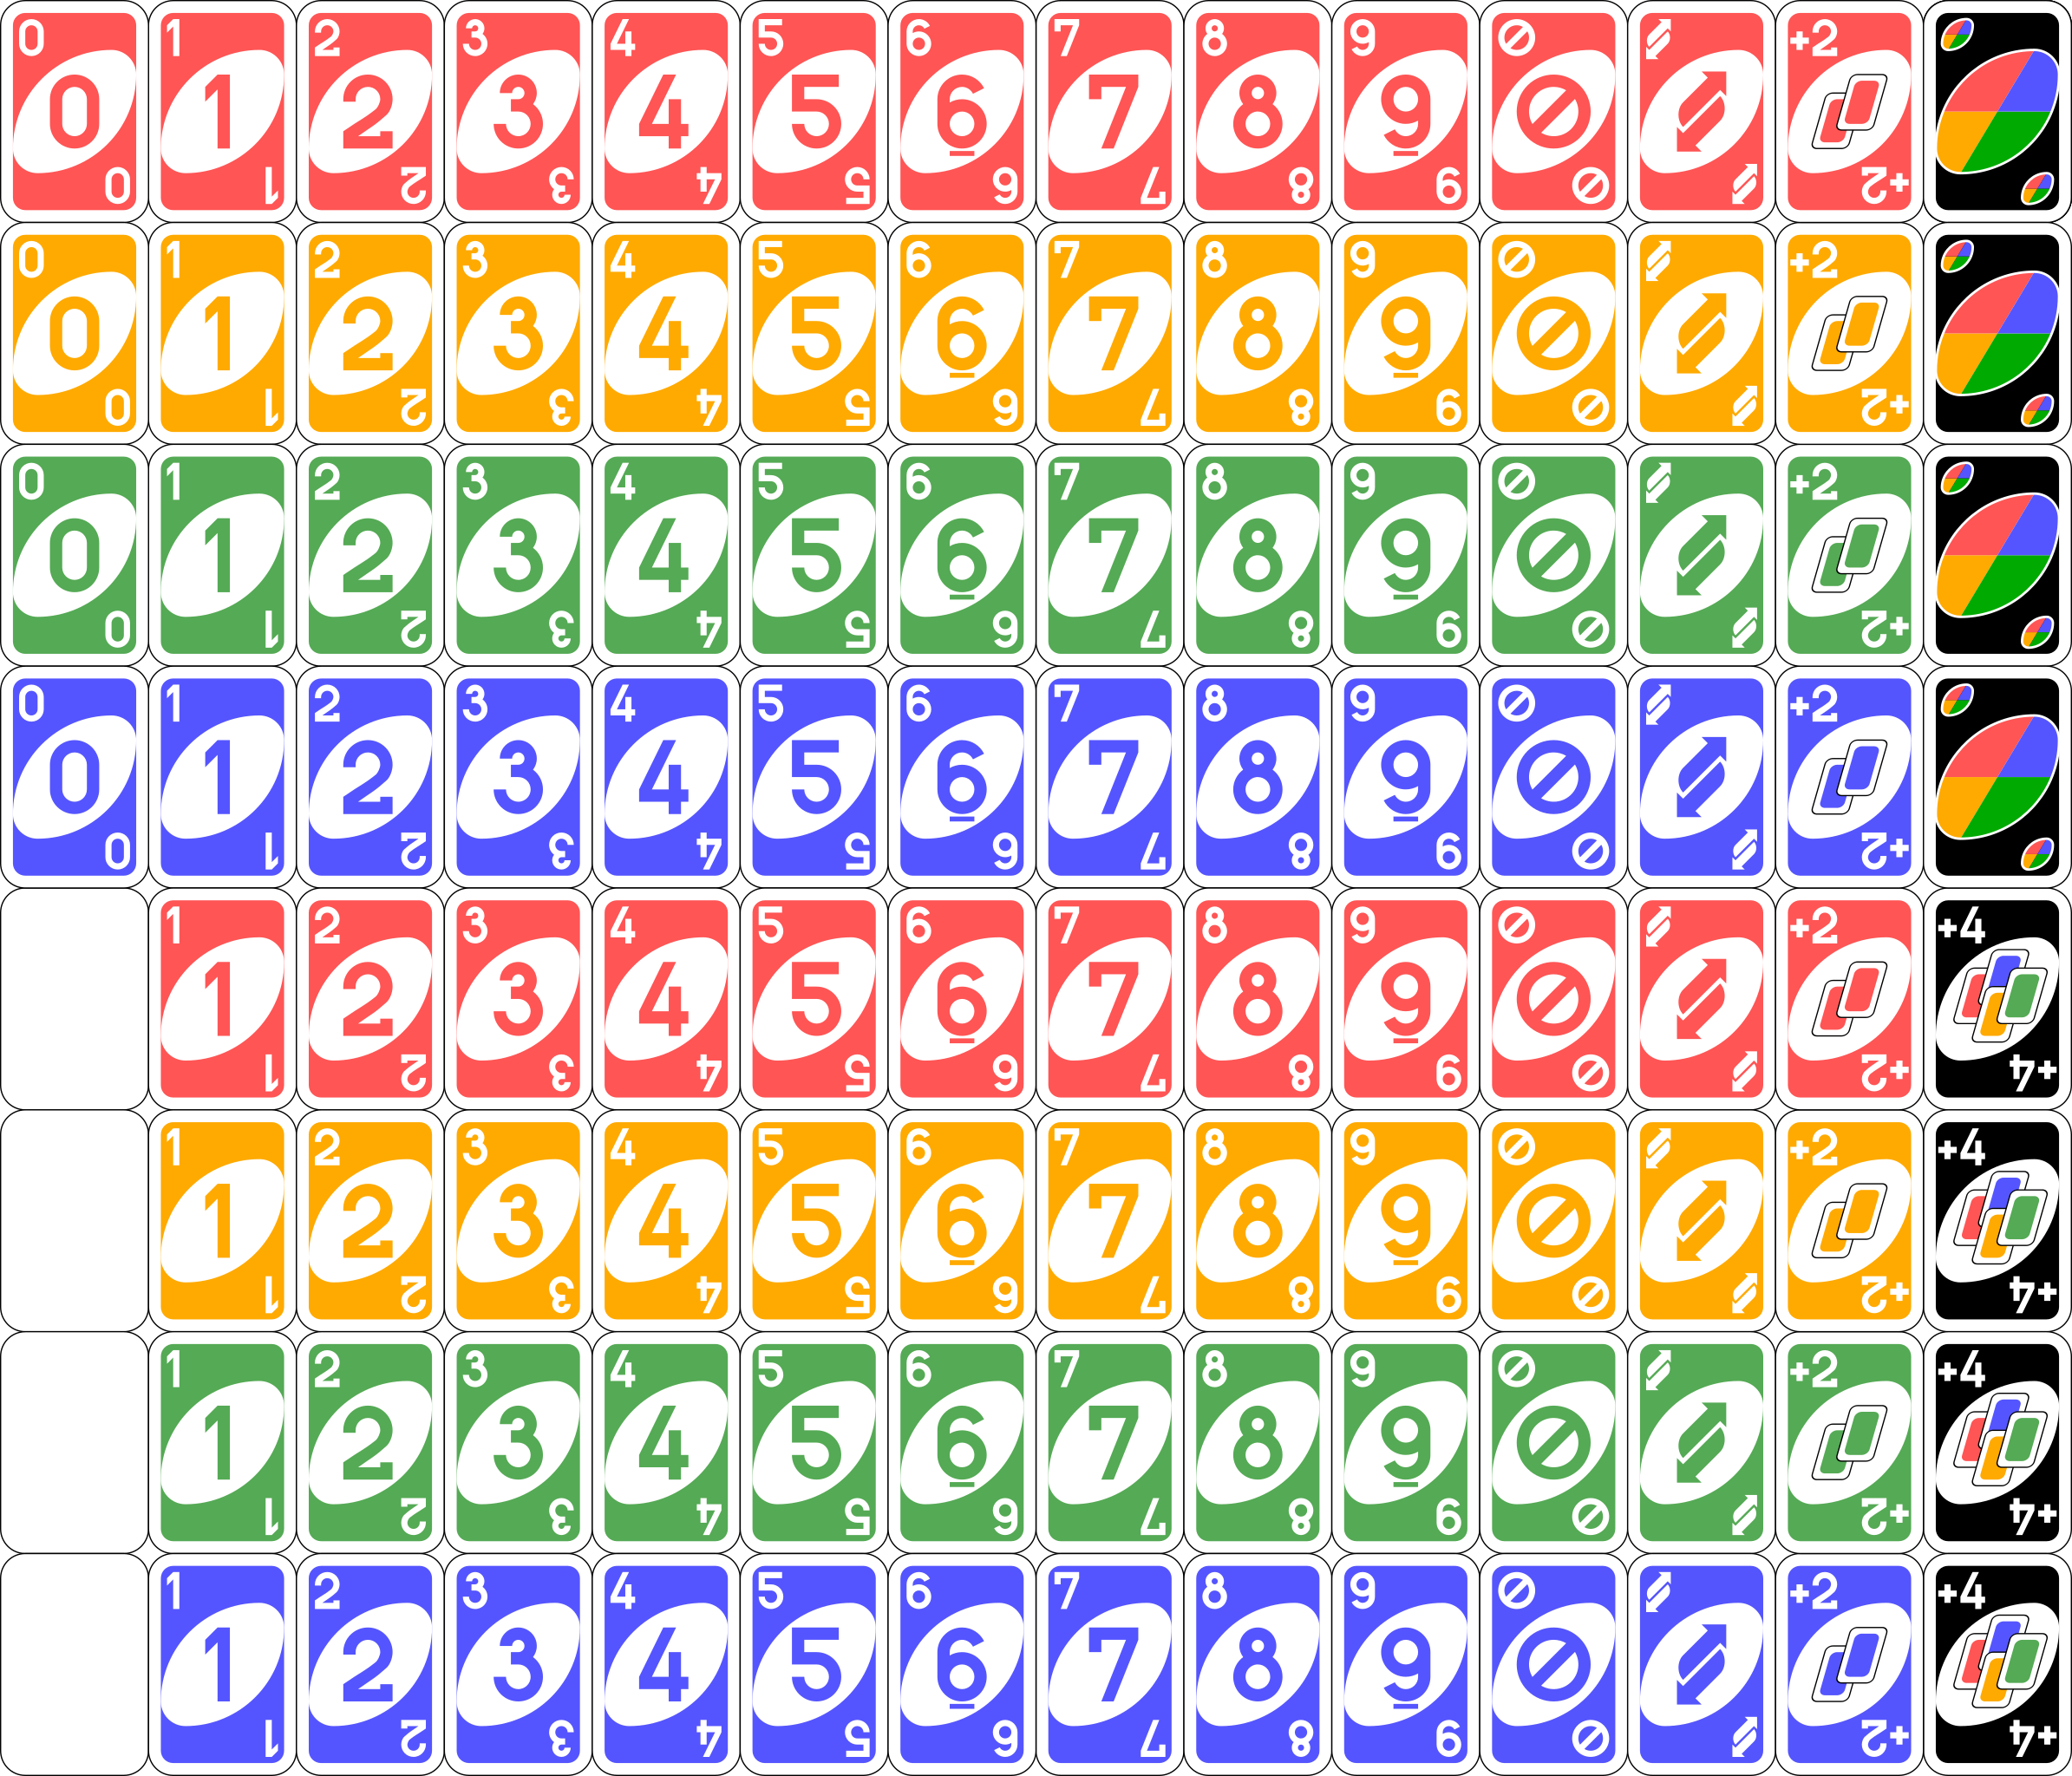
\includegraphics[width=.5\linewidth]{bilder/UNO_cards_deck.png}
	\caption{UNO Karten}
	\source{https://shopping.mattel.com/de-de/products/uno-kartenspiel-w2087-de-de}
	\label{fig:uno_cards}
	%Quelle:  https://upload.wikimedia.org/wikipedia/commons/thumb/9/95/UNO_cards_deck.svg/2389px-UNO_cards_deck.svg.png
\end{center}
\end{figure}
Die einfachen Karten existieren in vier verschiedenen Farben. Jede Farb-Zahl-Kombination existiert zweimal, wobei die Karten mit einer null nur einmal existieren. Im Rahmen dieser Arbeit sind vorrangig nur die einfachen Karten von Bedeutung. Spezialkarten verändern das Spielgeschehen, indem zum Beispiel der nächste Spieler für eine Runde aussetzen muss, oder zwei Karten ziehen muss. \\
Zu Beginn des Spiels erhält jeder Spieler 7 Karten. In der Tischmitte wird eine Karte aufgedeckt platziert, auf dem die Spieler nach der Reihe Karten ablegen oder ziehen können. Im Folgenden wird auf die Spielregeln eingegangen, die für das Ablegen von Karten gelten.
\section{Spielregeln}
Ziel einer Runde ist es, als erster Spieler alle Handkarten auf den in der Tischmitte platzierten Kartenstapel abzulegen. Daraufhin werden die Wertungen der Karten der Gegenspieler addiert und dem Gewinner der Runde als Punkte gutgeschrieben. Der erste Spieler, der 500 Punkte erreicht, gewinnt das Spiel. Die Spieler sind nacheinander im Uhrzeigersinn an der Reihe. Eine Karte kann abgelegt werden, wenn entweder die Zahl oder die Farbe der abzulegenden Karte mit der Zahl oder Farbe der in der Tischmitte liegenden Karte übereinstimmt. Hat der Spieler keine passende Karte auf der Hand, so muss er eine neue Karte vom Stapel ziehen. Der Zug ist damit beendet. Hat ein Spieler nur noch eine Karte auf der Hand, so muss er dies mit dem Wort \textit{UNO} den anderen Spielern mitteilen. Wird die letzte Karte ohne diese Aussage abgelegt, so muss die Karte wieder aufgenommen und eine Strafkarte vom Stapel gezogen werden. Daraufhin ist der Zug beendet \cite{UnoRules}. Die Regeln bezüglich der Spezialkarten sind im Rahmen dieser Arbeit nicht von Bedeutung.
%!TEX root = Uno-Dokumentation.tex

\chapter{Software}

\section{Grundlegender Aufbau}
In diesem Kapitel wird auf den Aufbau der gesamten Software eingegangen und soll einen Überblick über das Projekt geben. Abbildung \ref{fig:aufbau} zeigt die Menüführung der Software als Blockdiagramm. 
\begin{figure}[h]
	\begin{center}
		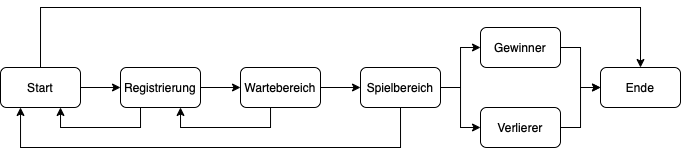
\includegraphics[width=\linewidth]{Uno_Pages.png}
		\caption{Blockdiagramm Software-Aufbau}
		\label{fig:aufbau}
	\end{center}
\end{figure}
Wird die Software gestartet, so wird die Startseite aufgerufen. Hier kann der Spieler das Spiel beenden, starten oder die Spielregeln einsehen. Wird das Spiel gestartet öffnet sich die Registrierungsseite. Hier wird der Spieler dazu aufgefordert seinen Namen einzugeben. Der Name wird dazu verwendet, um später im Spiel zu identifizieren welcher Spieler gerade am Zug ist. Für die Eingabe des Namens steht ein Textfeld zur Verfügung, welches auf maximal 20 einzugebende Zeichen begrenzt ist. Startet der Spieler das Spiel, so wird standardmäßig versucht eine Verbindung zu einem bestehenden Server aufzubauen. Wird jedoch ein Häkchen auf der Registrierungsseite gesetzt, so kann ein neuer Server gestartet werden. Nach der Registrierung wird der Spieler in einen Wartebereich geleitet. Dort wird auf die anderen drei Spieler gewartet. Entsprechende Benutzerrückmeldungen zeigen den aktuellen Status der Netzwerkverbindung und neu verbundene oder getrennte Spieler. Der Wartebereich wird automatisch verlassen, wenn vier Spieler erfolgreich mit dem Server verbunden sind. Ist dies der Fall, öffnet sich der Spielbereich. In diesem Bereich wird das Spiel gespielt. Je nach dem ob der Spieler die Runde gewinnt oder verliert, öffnet sich eine entsprechende Seite, auf der das Ergebnis gezeigt wird. Bei den Spielern, die verloren haben, wird der Name des Spielers gezeigt der die Runde gewonnen hat. Die Software kann an diesem Punkt nur noch beendet werden. Um eine neue Runde zu starten muss auch die Software neu gestartet werden.
\section{Klassen}

\subsection{GameServer}
Der \textit{GameServer} ist das Herzstück des ganzen Spiels. Er verarbeitet jegliche Spiellogik und Anfragen von Clients. Im folgenden wird genauer auf die Klasse eingegangen.\\
Für die Server-Client-Verbindungen wird ein sogenanntes \textit{NuGet-Paket} verwendet, welches compilierten Code enthält, der in externen Projekten verwendet werden kann \cite{NuGet}. Im Rahmen dieser Arbeit wird das \textit{SuperSimpleTCP}-Paket verwendet. Es enthält alle Klassen und Methoden, um einfache Server-Client-Verbindungen über das TCP-Protokoll herzustellen.\\
%TODO TCP acro
Codeausschnitt \ref{code:gameserver} zeigt einen Ausschnitt der \textit{GameServer}-Klasse. Es handelt sich dabei um eine statische Klasse, da der Server zu jedem Zeitpunkt verfügbar sein muss und nur eine einzige Instanz der Klasse benötigt wird. Der Klassen-Member \textit{server} beinhaltet alle Server-Funktionalitäten. Mit der Methode \textit{StartServer()} wird ein neuer Server gestartet und die Event-Methoden in Zeile 11 - 13 an die entsprechenden Server-Events angefügt. Wird nun ein Datenpaket empfangen, so wird ein neuer Thread gestartet, indem das eingehende Datenpaket entsprechend seines Inhalts verarbeitet wird. Die private Klasse \textit{RxMsg} dient zur Verarbeitung der Nachricht. Mit der Methode \textit{Stop()} werden aktive Verbindungen getrennt und der Server gestoppt.
\begin{lstlisting}[label={code:gameserver}, caption={Codeausschnitt Klasse \textit{GameServer}}]
	static class GameServer
	{
		static private SimpleTcpServer server;
		static private CardStack AllCards;
		static private CardStack MiddleStack;
		static private List<Player> AllPlayers = new List<Player>();
		static private int activePlayer = 0;
		
		static public bool StartServer();
		
		private static void Events_DataReceived(object? sender, DataReceivedEventArgs e);
		private static void Events_ClientDisconnected(object? sender, ConnectionEventArgs e);
		private static void Events_ClientConnected(object? sender, ConnectionEventArgs e);
		
		public static void serverBroadcast(string msg);
		public static void Stop();
		public static void StartGame();
		private static void removePlayer(string IpPort);
		public static bool isActive();
		
		private class RxMsg;
		{
			public string addPlayer(string name, string IpPort);
			public void removePlayer(string IpPort);
			private string CheckDuplicateNames(string name);
			private bool checkMovePossibility(int number, int color);
		}
	}
	
\end{lstlisting}
\subsection{Client}
\subsection{Card / CardStack}
Die Spielkarten spielen eine essentielle Rolle. Aus diesem Grund werden zwei Klassen für den Umgang mit den einzelnen Karten (\textit{Card}) und einem Kartenstapel (\textit{CardStack}) verwendet. Zunächst wird die Klasse \textit{Card} für eine einzelne Karte betrachtet. Wie in Kapitel \ref{ch:bedingungen} beschrieben, werden nur einfache Karten programmiert. Sie bestehen aus einer Farbe, repräsentiert durch einen ganzzahligen Zahlenwert zwischen null und drei und einer Zahl zwischen null und neun. Codeausschnitt \ref{code:card} zeigt einen Ausschnitt der Klasse \textit{Card}. Weitere Attribute werden für eine einfache Karte nicht benötigt. Die Klasse kann jedoch erweitert werden um Spezialkarten repräsentieren zu können.
\begin{lstlisting}[label={code:card}, caption={Codeausschnitt Klasse \textit{Card}}]
	public class Card
	{
		public int number;
		public int color;
		
		public Card(int number, int color)
		{
			this.number = number;
			this.color = color;
		}
	}
\end{lstlisting}
Codeausschnitt \ref{code:stack} zeigt den grundsätzlichen Aufbau der \textit{CardStack}-Klasse. Ein Karten-Stapel (CardStack) besteht aus einer Liste (\textit{Cards}) mit Elementen des Typs \textit{Card}. Zu beginn eines Spiels werden mithilfe der Methode \textit{createAllCards()} alle möglichen Spielkarten, wie in Kapitel \ref{ch:karten} beschrieben zu der Liste \textit{Cards} hinzugefügt. Um eine Karte zu ziehen, wird die Methode \textit{getRandomCard()} verwendet. Die Methode gibt eine zufällig gewählte Karte zurück und entfernt sie aus dem Stapel. Mithilfe der Methode \textit{returnCard(int index)} kann eine Karte an einer spezifischen Stelle des Stapels erhalten werden. Ein Karte kann dem Stapel mit der Methode \textit{AddCard(Card add)} hinzugefügt und mit \textit{RemoveCard(Card rem)} entfernt werden. Eine Karte kann nur entfernt werden, wenn sie in der Liste vorhanden ist. Ist die Karte nicht in der Liste vorhanden, so ist der Rückgabewert der Methode \textit{null}. Die Anzahl der Karten im Stapel wird mit der Methode \textit{getCounter()} zurückgegeben.
\begin{lstlisting}[label={code:stack}, caption={Codeausschnitt Klasse \textit{CardStack}}]
	public class CardStack
	{
		public List<Card> Cards { get; set; }
		public CardStack()
		{
			this.Cards = new List<Card>();
		}
	
		public void createAllCards();
		public Card getRandomCard();
		public Card returnCard(int index);
		public void AddCard(Card add);
		public Card RemoveCard(Card rem);
		public int getCounter();
	}
\end{lstlisting}

\subsection{Player}

%!TEX root = Uno-Dokumentation.tex

\chapter{Zusammenfassung}
Das Ziel des Projektes war es ein im Netzwerk spielbares Mehrspieler Spiel Uno zu programmieren. Da das Projekt nur von einer Person, anstatt von angedachten sechs Personen bearbeitet werden konnte, mussten einige Einschränkungen in Betracht gezogen werden. Eine einfache Spiellogik, nur grundlegende Regeln und Karten des Spiels und eine einfache, zweitrangige Optik. Die Anfangs gesetzten Haupt- und Nebenanforderungen sind im Verlauf des Projektes erfüllt worden. Resultat des Projektes ist ein mit vier Spielern spielbares Spiel. Es kann im Netzwerk von unterschiedlichen Rechnern aus zusammen gespielt werden. Grundlegende Spiellogik für einfache Karten, ausgenommen von Spezialkarten, lassen erkennen, dass es sich bei dem Spiel um Uno handelt. Die Objektorientierte und strukturierte Programmierung der Software lässt andere Entwickler schneller den Code verstehen und gibt die Möglichkeit für Erweiterungen und Optimierungen. Eine einfache, aber intuitive Menüführung der gesamten Software bedarf keiner Erklärung für den Benutzer. Optisch bietet sich noch viel Optimierungsbedarf, wobei die Kernelemente für den Benutzer verständlich angeordnet und beispielsweise die Karten farbig sind. Der Fokus der Programmierung lag jedoch von Anfang an auf der Funktion und nicht der Optik.\\
Durch die Verwendung verschiedenster Tools für die strukturierte Programmierung eines solchen Projekts konnte viel gelernt werden. Über Planung, Umsetzung, Versionsverwaltung und die Programmierung selbst. Das Projekt hat einen Einblick in die Arbeitsweise von Software-Entwicklern gegeben. Leider ist der Einblick in das Arbeiten im Team aufgrund von mangelnden Team-Mitgliedern zu kurz gekommen. Eine ungefähre Vorstellung konnte trotzdem erlangt werden.
%!TEX root = Uno-Dokumentation.tex
\chapter{Ausblick}
Das Projekt bietet einige Optimierungs- und Verbesserungspotential. Die Optik der Software ist noch auf keinem marktreifen Zustand und kann durch ein einheitliches Design, welches sich auf allen Seiten wiederfindet erheblich verbessert werden. Animationen, beispielsweise beim Ablegen einer Karte kann den Benutzern helfen die Spielzüge besser nachzuvollziehen. Neben der optischen Seite, kann auch der Code optimiert werden. Überflüssige Klassenmember und Methoden können entfernt werden, Und weitere Klassen können den Code besser verständlich und weniger komplex machen. Durch die objektorientierte Programmierung kann der Code einfach erweitert und optimiert werden. Zahlreiche Kommentare an nahezu jeder Methode, geben Entwicklern, die den Code zuvor noch nicht gesehen haben, die Möglichkeit ihn zu verstehen und weiterzuentwickeln. Die Client-Server-Verbindungen könnte optimiert werden, damit jedes Spiel zuverlässig funktioniert.\\
Die feste Anzahl von Spielern schränkt das Spielerlebnis erheblich ein. Mit einer Auswahl am Anfang des Spiels könnte der Spieler, der als Server agiert, festlegen mit wie viel Spielern das Spiel zu spielen ist. Dabei ist eine Anzahl laut der Regeln von zwei bis zehn Spielern sinnvoll \cite{Mattel}.

\printbibliography
\input{kapitel/Anhang.tex}

\end{document}          
